% 0. Baseline models
% 1. Blinding is easy enough to understand
% 2. The doubling of the action space - that's the brilliance
%

\subsection{Replicating Learning to navigate}

Since \cite{MiPaViICLR2017} did not release their source code, so we implemented their pipeline starting from \texttt{universe-start-agent}\cite{OpenAI2017UniverseStarterAgent}.

To make sure that we replicate \cite{MiPaViICLR2017} results, we setup the experiment as similar to what was described in the paper.
But unlike, \cite{MiPaViICLR2017} instead of hand picking the maps to run experiments on, we chose to run the experiments on randomly generated maps.
We create a set of randomly generated maps by a textbook depth first search based algorithm with randomly introduced loops.
\hl{Based on results chose one}
In our experiments, we found that we do not reach the latency scores of \cite{MiPaViICLR2017} but we reach close enough.
\hl{OR}
Results in Table~\ref{tab:TODO} establish conclusively that the NavA3C agents replicated by us do perform at least as well as the agents .
%%%%%
Note, that we report standard deviation over latency metric which indicates that the variation between maps and algorithm is not significant enough to overcome the variation within the maps.
This shows that the experiments in \cite{MiPaViICLR2017} were not strong enough to support the hypothesis of learning to navigate.

\begin{table}[h]
    \label{sample-table}
    \begin{center}
        \begin{tabular}{llll}
          \toprule
          Training maps & Reward & Latency 1:$>1$ & Goals \\
          \midrule
          1 & 41.01 $\pm$  16.78 & 152.3:145.3 $\pm$ 118.88:83.95 & 3.48 $\pm$ 1.65 \\
          10 & 30.89 $\pm$  20.87 & 154.05:156.86 $\pm$ 140.03:98.26 & 2.47 $\pm$ 1.72 \\
          1000 & 40.27 $\pm$  20.47 & 148.20:148.12 $\pm$ 130.45:95.28 & 3.14 $\pm$ 1.89 \\
          \bottomrule
        \end{tabular}
    \end{center}
    \caption{We achieve comparable results when we test and train on the same experiments.}
\end{table}

\subsection{Training on multiple maps}
Can we generalize the performance of the agent by training on multiple maps? The answer turns out to be no.

\subsection{Evaluation on unseen maps}
What if we test on unseen maps, will the agents be able to tranfer their strategies onto unseen maps? The answer turns out to be no.

\subsection{Do the agents learn a frame to action mapping and repeat it?}
NO
\hl{Show qualitative and quantitative results to address this hypothesis}

\subsection{Do the agents memorize the path and repeat it?}
NO
\hl{Show qualitative and quantitative results to address this hypothesis}

\subsection{Are these agent doing better path planning than random?}
We evaluate the trained agents on 1000 random maps on very simple maps which have only two possible paths to reach the goal -- one shorter than the other. We evaluate the agent whether it does better than a random agent.
It does not.

We propose a 5-stage benchmark for reinforcement learning based methods to takeover the navigation problem.
\begin{enumerate}
  \item Train to find optimal path on the same map with fixed goal.
  \item Train to find optimal path on the same map with varying goal. 
    \begin{enumerate}
    \item Explore different paths, remember the shortest path and repeat it.
    \item Explore different paths, learn frame to action mapping to follow the shortest path from any point.
    \item Explore different paths, learn to compute and follow optimal path.
    \end{enumerate}
  \item Train to find optimal path on the unseen map with varying goal. 
\end{enumerate}

\begin{figure}
 \vspace{-3em}%
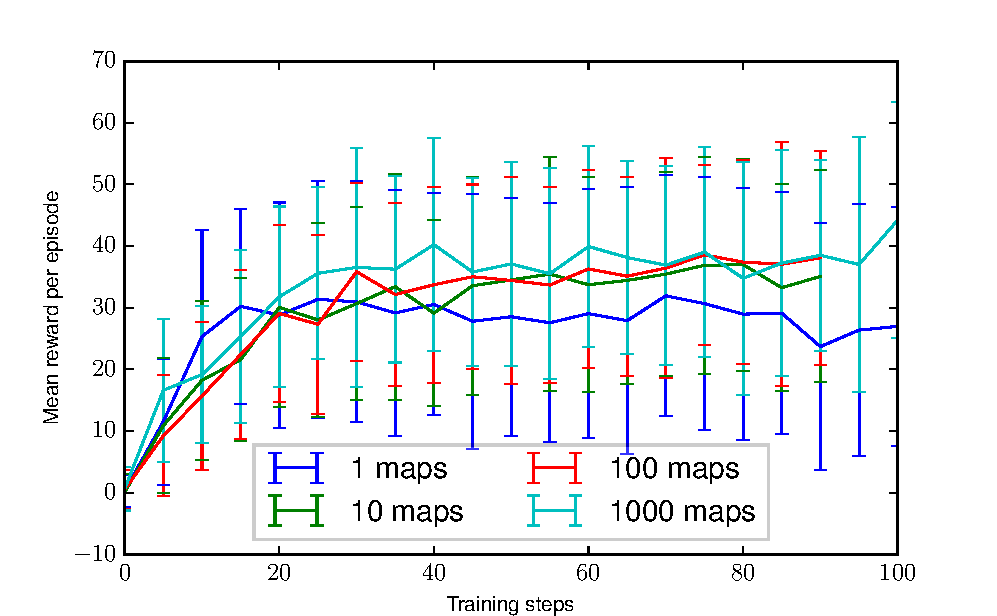
\includegraphics[width=0.5\columnwidth]{images/plot_reward_3D-1000.pdf}%
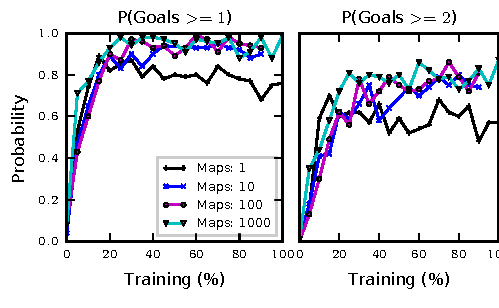
\includegraphics[width=0.5\columnwidth]{images/plot_probability_3D-1000.pdf}%
\vspace{-1em}%
\caption{Mean reward while tested on 100 unseen maps, while being trained on different number of training maps. Note that while training on 1000 maps eventually achieves high reward, it is only higher mean reward (44.2), training on 1 map hits the maximum (31) much faster.}
\label{fig:plot_reward_on_testing}
\end{figure}

